\documentclass[12pt, hidelinks]{article}
\usepackage[brazil]{babel}
\usepackage[utf8]{inputenc}
\usepackage{amsmath}
\usepackage{natbib}
\usepackage{listings}
\usepackage{color}

\definecolor{codegreen}{rgb}{0,0.6,0}
\definecolor{codegray}{rgb}{0.5,0.5,0.5}
\definecolor{codepurple}{rgb}{0.58,0,0.82}
\definecolor{backcolour}{rgb}{0.95,0.95,0.92}

\lstdefinestyle{mystyle}{
  backgroundcolor=\color{backcolour},
  commentstyle=\color{codegreen},
  keywordstyle=\color{red},
  numberstyle=\tiny\color{codegray},
  stringstyle=\color{codepurple},
  basicstyle=\footnotesize,
  breakatwhitespace=false,
  breaklines=true,
  captionpos=b,
  keepspaces=true,
  numbers=left,
  numbersep=5pt,
  showspaces=false,
  showstringspaces=false,
  showtabs=false,
  tabsize=2,
  extendedchars=true,
  literate={á}{{\'a}}1 {ã}{{\~a}}1 {õ}{{\~o}}1 {é}{{\'e}}1 {ç}{{\c{c}}}1,
}

\lstset{style=mystyle}
\usepackage{url}
\usepackage{amsmath}
\usepackage{float}
\usepackage{graphicx}
\graphicspath{{images/}}
\usepackage{parskip}
\usepackage{fancyhdr}
\usepackage{vmargin}
\usepackage{hyperref}
\setmarginsrb{3 cm}{2.5 cm}{3 cm}{2.5 cm}{1 cm}{1.5 cm}{1 cm}{1.5 cm}


\title{Integração Numérica}         % Title
\author{Wilton Rodrigues}								% Author
\date{\today}											      % Date

\makeatletter
\let\thetitle\@title
\let\theauthor\@author
\let\thedate\@date
\makeatother

\pagestyle{fancy}
\fancyhf{}
\lhead{\centering{\thetitle}}
\cfoot{\thepage}

\begin{document}

%%%%%%%%%%%%%%%%%%%%%%%%%%%%%%%%%%%%%%%%%%%%%%%%%%%%%%%%%%%%%%%%%%%%%%%%%%%%%%%%%%%%%%%%%

\begin{titlepage}
  \centering
  \begin{figure}[H]
    \centering
    
\includegraphics[width=0.7\textwidth]{figuras/logo.png}\\[2.0 cm]
  \end{figure}
  \textsc{\LARGE Universidade de Brasília}\\[2.5 cm]	% University Name
  \textsc{\Large Relatório de atividade do módulo 5}\\[0.5 cm]				% Activity name
  \textsc{\large Métodos Numéricos para Engenharia}\\[1.5 cm]				% Course Name
  \rule{\linewidth}{0.2 mm} \\[0.4 cm]
  {\huge \bfseries \thetitle}\\
  \rule{\linewidth}{0.2 mm} \\[2.5 cm]

  \begin{minipage}{0.4\textwidth}
    \begin{flushleft} \large
      \emph{Aluno:}\\
      \theauthor
    \end{flushleft}
  \end{minipage}
  \begin{minipage}{0.4\textwidth}
    \begin{flushright} \large
      \emph{Matrícula:} \\
      13/0049212									% Your Student Number
    \end{flushright}
  \end{minipage}\\
  \vspace*{0.5in}
  {\large \thedate}\\[0.5 cm]

  \vfill

\end{titlepage}

%%%%%%%%%%%%%%%%%%%%%%%%%%%%%%%%%%%%%%%%%%%%%%%%%%%%%%%%%%%%%%%%%%%%%%%%%%%%%%%%%%%%%%%%%

\section{Introdução}

O objetivo deste relatório é exercitar os conceitos aprendidos em aula, com relação ao tópico: \thetitle.

Em determinadas situações, integrais são difíceis, ou mesmo impossíveis de se resolver analiticamente. Para contornar esse obstáculo é possível, através da substituição da função $f(x)$ por um polinômio que a aproxime razoavelmente num dado intervalo $[a, b]$, encontrar o valor da integral.

O problema a ser solucionado é o que trata da função seno integral, como é mostrado a seguir:

\begin{eqnarray}\label{eq:integral}
  Si(x) = \int_{0}^{x} \frac{sen(t)}{t}dt
\end{eqnarray}

Onde o objetivo deste relatório será, através do método da regra do trapézio composta, plotar o gráfico da equação~\eqref{eq:integral} com $100$ valores de $x$ no intervalo $0 < x < 10$, além de calcular os valores de $Si(0,5)$ e $Si(5,5)$ com precisão de $6$ casas decimais.

\section{Metodologia}
Baseando-se no método da Regra do Trapézio composta, como dito anteriormente, tem-se a seguinte relação:
\begin{eqnarray}\label{eq:trapezio}
  \int_{x_0}^{x_n} f(x)dx = \sum\limits_{i=0}^{n-1}\int_{x_i}^{x_{i+1}} f(x)dx = \sum\limits_{i=0}^{n-1}\frac{h}{2}[f(x_i) + f(x_{i+1})]
\end{eqnarray}
Onde podemos escrever a equação~\eqref{eq:trapezio} como:
\begin{eqnarray}\label{eq:trapcomposta}
  \int_{x_0}^{x_n} f(x)dx = \frac{h}{2}[f(x_0) + f(x_1) + \hdots + f(x_{n-1}) + f(x_n)]
\end{eqnarray}

Como o problema especifica uma quantidade mínimia de pontos a serem apresentados, a qual vamos chamar de $N$, o nosso $h$ será calculado de acordo com a seguinte relação:
\begin{eqnarray}\label{eq:h}
  h = (x_n - x_0)/N
\end{eqnarray}

% \begin{table}[h]
%   \centering
%   \begin{tabular}{|c|c|c|c|c|c|c|c|c|c|}
%     \hline
%       $T$ & 0 & 5 & 10 & 15 & 20 & 25 & 30 & 35 & 40\\
%     \hline
%       $\rho$ & 0.9999 & 0.9998 & 0.9997 & 0.9991 & 0.9982 & 0.9971 & 0.9957 & 0.9941 & 0.9902\\
%     \hline
%   \end{tabular}
%   \caption{Valores tabelados}
%   \label{tab:tabeladados}
% \end{table}

\newpage
\section{Diagrama esquemático de execução}
Nesta seção, encontra-se o fluxo de execução utilizando a linguagem C. Que é apresentada na próxima sessão.
\begin{figure}[!h]
  \centering
  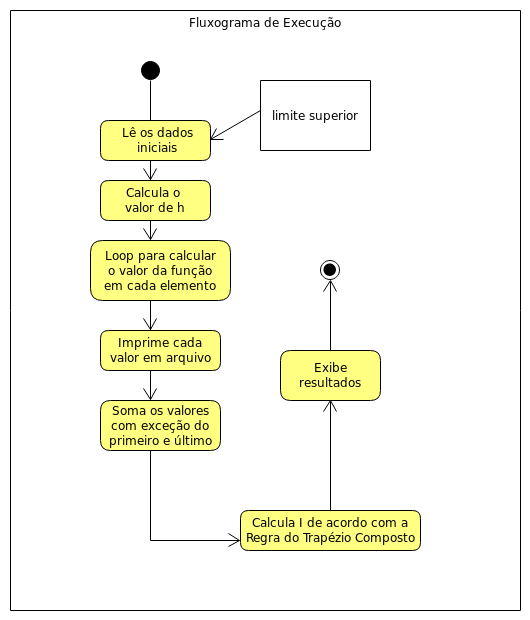
\includegraphics[width=10cm]{figuras/fluxograma.png}\\
  \caption{Fluxo de execução da solução}\label{fig:fluxo}
\end{figure}
A solução elaborada neste relatório funciona da seguinte maneira. É necessário inserir o limite superior através da linha de comando. O programa trabalha com uma quantidade fixa de $100$ elementos para fazer a aproximação do resultado.
Primeiramente o programa calcula o valor do $h$ de acordo com a equação~\eqref{eq:h}. Após isso o programa entra em um loop no qual ele calcula os intervalos, $h$, e atribui para cada um deles o valor resultante da função $Sin(x)/x$. Juntamente com isto, o programa já gera um arquivo, que será utilizado mais a frente para gerar o gráfico da função, com os pontos da equação e os respectivos valores. Em seguida são somados todos os elementos com exceção do primeiro e último. Após isto calcula-se o valor de $I$ de acordo com a Regra do Trapézio Composto. Por fim é apresentado o resultado em tela.

\newpage
\section{Código Fonte}\label{sec:codigofonte}

\lstinputlisting[language=C]{../solution/m5.c}

\newpage
\section{Resultados e discussões}

Nesta seção discutiremos os resultados obtidos após a execução do programa apresentado na seção anterior.

Primeiramente, será apresentada a plotagem do gráfico da equação~\eqref{eq:integral} para o intervalo $[0, 10]$, como havia sido estabelecido no início do relatório. Para gerar estes pontos, basta executar o programa com o limite superior $= 10$. Um arquivo será gerado com todos os pontos e os respectivos valores. Então, através da ferramenta Gnuplot, foi feita a plotagem do gráfico.
\begin{figure}[!h]
  \centering
  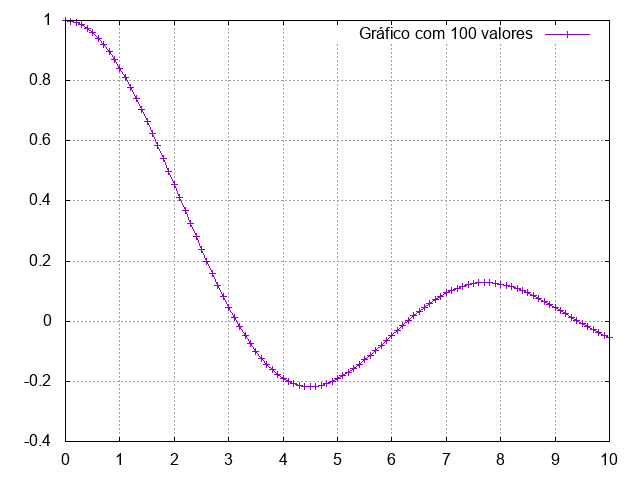
\includegraphics[width=15cm]{figuras/graph.png}\\
  \caption{Plotagem de 100 valores no intervalo $[0,10]$ }\label{fig:graph}
\end{figure}
\newpage
Após isso, executou-se o programa para os valores $Si(0,5)~e~Si(5,5)$:
\begin{figure}[!h]
  \centering
  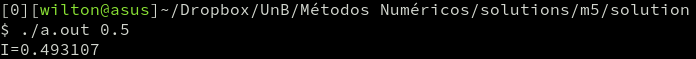
\includegraphics[width=15cm]{figuras/si05.png}\\
  \caption{Resultado da execução do programa para $Si(0,5)$}\label{fig:printro13}
\end{figure}

\begin{figure}[!h]
  \centering
  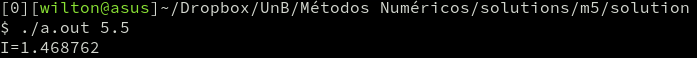
\includegraphics[width=15cm]{figuras/si55.png}\\
  \caption{Resultado da execução do programa para $Si(5,5)$}\label{fig:printro27}
\end{figure}
Após a execução do programa foram obtidos os seguintes valores:
$$Si(0,5) = 0.493107~e~Si(5,5) = 1.468762$$
Devido ao fato de o método utilizado ter sido a Regra do Trapézio Composto, para não cairmos em uma indeterminação ao aplicarmos o método ao primeiro elemento que resultaria em uma divisão por $0$, substituiu-se este valor por $1$x$10^{-8}$.

O resultado encontrado a partir da solução proposta é condizente. Pois ao fazermos a comparação dos valores obtidos com os resultados obtidos no site WolframAlpha (https://www.wolframalpha.com), chegamos ao mesmo resultado:

\begin{figure}[!h]
  \centering
  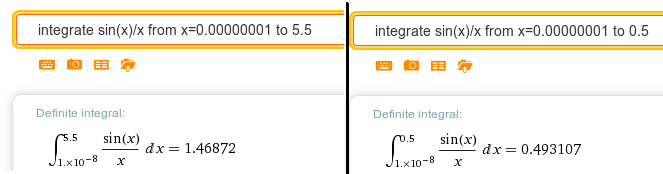
\includegraphics[width=15cm]{figuras/wolf.png}\\
  \caption{Resultados do WolframAlpha}
  \label{fig:w05}
\end{figure}

Sendo assim, o objetivo proposto no início do relatório foi satisfatoriamente alcançado.

\newpage
\section{Ferramentas}
Todas as ferramentas utilizadas neste relatório são ferramentas open source (software livre).
Permitindo assim que qualquer um possa reproduzir e contestar as afirmações presentes neste documento.

\begin{enumerate}
  \item Arch Linux (\url{https://www.archlinux.org})
    \begin{itemize}
      \item Sistema operacional utilizado.
    \end{itemize}
  \item GCC (\url{https://gcc.gnu.org})
    \begin{itemize}
      \item Compilador de C utilizado para compilar a solução.
    \end{itemize}
  \item Python (\url{https://www.python.org})
    \begin{itemize}
      \item Linguagem de programação utilizada para conferir os valores da solução.
    \end{itemize}
  \item vim (\url{http://www.vim.org})
    \begin{itemize}
      \item Editor de texto.
    \end{itemize}
  \item \LaTeX~(\url{https://www.latex-project.org})
    \begin{itemize}
      \item Sistema tipográfico de alta qualidade (utilizado para elaborar o relatório).
    \end{itemize}
  \item Gnuplot (\url{http://www.gnuplot.info})
    \begin{itemize}
      \item Utilitário de representação gráfica (utilizado para plotagem do gráfico).
    \end{itemize}
  \item UMLet (\url{http://www.umlet.com})
    \begin{itemize}
      \item Ferramenta de UML (utilizado para criar o fluxo de execução).
    \end{itemize}
  \item Shutter (\url{http://shutter-project.org})
    \begin{itemize}
      \item Programa de captura de tela (utilizado para capturar os resultados).
    \end{itemize}
\end{enumerate}

%%%%%%%%%%%%%%%%%%%%%%%%%%%%%%%%%%%%%%%%%%%%%%%%%%%%%%%%%%%%%%%%%%%%%%%%%%%%%%%%%%%%%%%%%

\end{document}
